\documentclass[a4paper, 12pt]{article}
\usepackage[brazil]{babel}
\usepackage{indentfirst}
\usepackage{graphicx}
\usepackage{graphics}

\usepackage{tabularx}
\usepackage{graphicx}
\usepackage{adjustbox}

\usepackage{booktabs}
\usepackage[font=footnotesize,labelfont=bf]{caption} %muda o tamanho das caption e deixa em negrito
\usepackage{cite}
\usepackage{color}   %May be necessary if you want to color links
\usepackage{hyperref}
\hypersetup{
    colorlinks=true,
    citecolor=blue,
    filecolor=blue,
    linkcolor=blue,
    urlcolor=blue
}
%%%%%%%%%%%%%%%%%%%%%%%%%%%%%%%%%%%%%%%%%%%%%%%%
%%%%%%%%%%%%%%%%%%%%JUPYTER TEX%%%%%%%%%%%%%%%%%
%%%%%%%%%%%%%%%%%%%%%%%%%%%%%%%%%%%%%%%%%%%%%%%%
\usepackage[breakable]{tcolorbox}
\tcbset{nobeforeafter} % prevents tcolorboxes being placing in paragraphs
\usepackage{float}
\floatplacement{figure}{H} % forces figures to be placed at the correct location

\usepackage[T1]{fontenc}
% Nicer default font (+ math font) than Computer Modern for most use cases
\usepackage{mathpazo}

% Basic figure setup, for now with no caption control since it's done
% automatically by Pandoc (which extracts ![](path) syntax from Markdown).
\usepackage{graphicx}
% We will generate all images so they have a width \maxwidth. This means
% that they will get their normal width if they fit onto the page, but
% are scaled down if they would overflow the margins.
\makeatletter
\def\maxwidth{\ifdim\Gin@nat@width>\linewidth\linewidth
\else\Gin@nat@width\fi}
\makeatother
\let\Oldincludegraphics\includegraphics
% Set max figure width to be 80% of text width, for now hardcoded.
% \renewcommand{\includegraphics}[1]{\Oldincludegraphics[width=.8\maxwidth]{#1}}
% Ensure that by default, figures have no caption (until we provide a
% proper Figure object with a Caption API and a way to capture that
% in the conversion process - todo).

% \usepackage{caption}
% \DeclareCaptionLabelFormat{nolabel}{}
% \captionsetup{labelformat=nolabel}

\usepackage{adjustbox} % Used to constrain images to a maximum size 
\usepackage{xcolor} % Allow colors to be defined
\usepackage{enumerate} % Needed for markdown enumerations to work
\usepackage{geometry} % Used to adjust the document margins
\usepackage{amsmath} % Equations
\usepackage{amssymb} % Equations
\usepackage{textcomp} % defines textquotesingle
% Hack from http://tex.stackexchange.com/a/47451/13684:
\AtBeginDocument{%
    \def\PYZsq{\textquotesingle}% Upright quotes in Pygmentized code
}
\usepackage{upquote} % Upright quotes for verbatim code
\usepackage{eurosym} % defines \euro
\usepackage[mathletters]{ucs} % Extended unicode (utf-8) support
\usepackage[utf8x]{inputenc} % Allow utf-8 characters in the tex document
\usepackage{fancyvrb} % verbatim replacement that allows latex
\usepackage{grffile} % extends the file name processing of package graphics 
                     % to support a larger range 
% The hyperref package gives us a pdf with properly built
% internal navigation ('pdf bookmarks' for the table of contents,
% internal cross-reference links, web links for URLs, etc.)
\usepackage{hyperref}
\usepackage{longtable} % longtable support required by pandoc >1.10
\usepackage{booktabs}  % table support for pandoc > 1.12.2
\usepackage[inline]{enumitem} % IRkernel/repr support (it uses the enumerate* environment)
\usepackage[normalem]{ulem} % ulem is needed to support strikethroughs (\sout)
                            % normalem makes italics be italics, not underlines
\usepackage{mathrsfs}



% Colors for the hyperref package
\definecolor{urlcolor}{rgb}{0,.145,.698}
\definecolor{linkcolor}{rgb}{.71,0.21,0.01}
\definecolor{citecolor}{rgb}{.12,.54,.11}

% ANSI colors
\definecolor{ansi-black}{HTML}{3E424D}
\definecolor{ansi-black-intense}{HTML}{282C36}
\definecolor{ansi-red}{HTML}{E75C58}
\definecolor{ansi-red-intense}{HTML}{B22B31}
\definecolor{ansi-green}{HTML}{00A250}
\definecolor{ansi-green-intense}{HTML}{007427}
\definecolor{ansi-yellow}{HTML}{DDB62B}
\definecolor{ansi-yellow-intense}{HTML}{B27D12}
\definecolor{ansi-blue}{HTML}{208FFB}
\definecolor{ansi-blue-intense}{HTML}{0065CA}
\definecolor{ansi-magenta}{HTML}{D160C4}
\definecolor{ansi-magenta-intense}{HTML}{A03196}
\definecolor{ansi-cyan}{HTML}{60C6C8}
\definecolor{ansi-cyan-intense}{HTML}{258F8F}
\definecolor{ansi-white}{HTML}{C5C1B4}
\definecolor{ansi-white-intense}{HTML}{A1A6B2}
\definecolor{ansi-default-inverse-fg}{HTML}{FFFFFF}
\definecolor{ansi-default-inverse-bg}{HTML}{000000}

% commands and environments needed by pandoc snippets
% extracted from the output of `pandoc -s`
\providecommand{\tightlist}{%
  \setlength{\itemsep}{0pt}\setlength{\parskip}{0pt}}
\DefineVerbatimEnvironment{Highlighting}{Verbatim}{commandchars=\\\{\}}
% Add ',fontsize=\small' for more characters per line
\newenvironment{Shaded}{}{}
\newcommand{\KeywordTok}[1]{\textcolor[rgb]{0.00,0.44,0.13}{\textbf{{#1}}}}
\newcommand{\DataTypeTok}[1]{\textcolor[rgb]{0.56,0.13,0.00}{{#1}}}
\newcommand{\DecValTok}[1]{\textcolor[rgb]{0.25,0.63,0.44}{{#1}}}
\newcommand{\BaseNTok}[1]{\textcolor[rgb]{0.25,0.63,0.44}{{#1}}}
\newcommand{\FloatTok}[1]{\textcolor[rgb]{0.25,0.63,0.44}{{#1}}}
\newcommand{\CharTok}[1]{\textcolor[rgb]{0.25,0.44,0.63}{{#1}}}
\newcommand{\StringTok}[1]{\textcolor[rgb]{0.25,0.44,0.63}{{#1}}}
\newcommand{\CommentTok}[1]{\textcolor[rgb]{0.38,0.63,0.69}{\textit{{#1}}}}
\newcommand{\OtherTok}[1]{\textcolor[rgb]{0.00,0.44,0.13}{{#1}}}
\newcommand{\AlertTok}[1]{\textcolor[rgb]{1.00,0.00,0.00}{\textbf{{#1}}}}
\newcommand{\FunctionTok}[1]{\textcolor[rgb]{0.02,0.16,0.49}{{#1}}}
\newcommand{\RegionMarkerTok}[1]{{#1}}
\newcommand{\ErrorTok}[1]{\textcolor[rgb]{1.00,0.00,0.00}{\textbf{{#1}}}}
\newcommand{\NormalTok}[1]{{#1}}

% Additional commands for more recent versions of Pandoc
\newcommand{\ConstantTok}[1]{\textcolor[rgb]{0.53,0.00,0.00}{{#1}}}
\newcommand{\SpecialCharTok}[1]{\textcolor[rgb]{0.25,0.44,0.63}{{#1}}}
\newcommand{\VerbatimStringTok}[1]{\textcolor[rgb]{0.25,0.44,0.63}{{#1}}}
\newcommand{\SpecialStringTok}[1]{\textcolor[rgb]{0.73,0.40,0.53}{{#1}}}
\newcommand{\ImportTok}[1]{{#1}}
\newcommand{\DocumentationTok}[1]{\textcolor[rgb]{0.73,0.13,0.13}{\textit{{#1}}}}
\newcommand{\AnnotationTok}[1]{\textcolor[rgb]{0.38,0.63,0.69}{\textbf{\textit{{#1}}}}}
\newcommand{\CommentVarTok}[1]{\textcolor[rgb]{0.38,0.63,0.69}{\textbf{\textit{{#1}}}}}
\newcommand{\VariableTok}[1]{\textcolor[rgb]{0.10,0.09,0.49}{{#1}}}
\newcommand{\ControlFlowTok}[1]{\textcolor[rgb]{0.00,0.44,0.13}{\textbf{{#1}}}}
\newcommand{\OperatorTok}[1]{\textcolor[rgb]{0.40,0.40,0.40}{{#1}}}
\newcommand{\BuiltInTok}[1]{{#1}}
\newcommand{\ExtensionTok}[1]{{#1}}
\newcommand{\PreprocessorTok}[1]{\textcolor[rgb]{0.74,0.48,0.00}{{#1}}}
\newcommand{\AttributeTok}[1]{\textcolor[rgb]{0.49,0.56,0.16}{{#1}}}
\newcommand{\InformationTok}[1]{\textcolor[rgb]{0.38,0.63,0.69}{\textbf{\textit{{#1}}}}}
\newcommand{\WarningTok}[1]{\textcolor[rgb]{0.38,0.63,0.69}{\textbf{\textit{{#1}}}}}


% Define a nice break command that doesn't care if a line doesn't already
% exist.
\def\br{\hspace*{\fill} \\* }
% Math Jax compatibility definitions
\def\gt{>}
\def\lt{<}
\let\Oldtex\TeX
\let\Oldlatex\LaTeX
\renewcommand{\TeX}{\textrm{\Oldtex}}
\renewcommand{\LaTeX}{\textrm{\Oldlatex}}
% Document parameters
% Document title
\title{Trabalho 1 - Intelig?ncia Artificial}





% Pygments definitions
\makeatletter
\def\PY@reset{\let\PY@it=\relax \let\PY@bf=\relax%
\let\PY@ul=\relax \let\PY@tc=\relax%
\let\PY@bc=\relax \let\PY@ff=\relax}
\def\PY@tok#1{\csname PY@tok@#1\endcsname}
\def\PY@toks#1+{\ifx\relax#1\empty\else%
\PY@tok{#1}\expandafter\PY@toks\fi}
\def\PY@do#1{\PY@bc{\PY@tc{\PY@ul{%
\PY@it{\PY@bf{\PY@ff{#1}}}}}}}
\def\PY#1#2{\PY@reset\PY@toks#1+\relax+\PY@do{#2}}

\expandafter\def\csname PY@tok@w\endcsname{\def\PY@tc##1{\textcolor[rgb]{0.73,0.73,0.73}{##1}}}
\expandafter\def\csname PY@tok@c\endcsname{\let\PY@it=\textit\def\PY@tc##1{\textcolor[rgb]{0.25,0.50,0.50}{##1}}}
\expandafter\def\csname PY@tok@cp\endcsname{\def\PY@tc##1{\textcolor[rgb]{0.74,0.48,0.00}{##1}}}
\expandafter\def\csname PY@tok@k\endcsname{\let\PY@bf=\textbf\def\PY@tc##1{\textcolor[rgb]{0.00,0.50,0.00}{##1}}}
\expandafter\def\csname PY@tok@kp\endcsname{\def\PY@tc##1{\textcolor[rgb]{0.00,0.50,0.00}{##1}}}
\expandafter\def\csname PY@tok@kt\endcsname{\def\PY@tc##1{\textcolor[rgb]{0.69,0.00,0.25}{##1}}}
\expandafter\def\csname PY@tok@o\endcsname{\def\PY@tc##1{\textcolor[rgb]{0.40,0.40,0.40}{##1}}}
\expandafter\def\csname PY@tok@ow\endcsname{\let\PY@bf=\textbf\def\PY@tc##1{\textcolor[rgb]{0.67,0.13,1.00}{##1}}}
\expandafter\def\csname PY@tok@nb\endcsname{\def\PY@tc##1{\textcolor[rgb]{0.00,0.50,0.00}{##1}}}
\expandafter\def\csname PY@tok@nf\endcsname{\def\PY@tc##1{\textcolor[rgb]{0.00,0.00,1.00}{##1}}}
\expandafter\def\csname PY@tok@nc\endcsname{\let\PY@bf=\textbf\def\PY@tc##1{\textcolor[rgb]{0.00,0.00,1.00}{##1}}}
\expandafter\def\csname PY@tok@nn\endcsname{\let\PY@bf=\textbf\def\PY@tc##1{\textcolor[rgb]{0.00,0.00,1.00}{##1}}}
\expandafter\def\csname PY@tok@ne\endcsname{\let\PY@bf=\textbf\def\PY@tc##1{\textcolor[rgb]{0.82,0.25,0.23}{##1}}}
\expandafter\def\csname PY@tok@nv\endcsname{\def\PY@tc##1{\textcolor[rgb]{0.10,0.09,0.49}{##1}}}
\expandafter\def\csname PY@tok@no\endcsname{\def\PY@tc##1{\textcolor[rgb]{0.53,0.00,0.00}{##1}}}
\expandafter\def\csname PY@tok@nl\endcsname{\def\PY@tc##1{\textcolor[rgb]{0.63,0.63,0.00}{##1}}}
\expandafter\def\csname PY@tok@ni\endcsname{\let\PY@bf=\textbf\def\PY@tc##1{\textcolor[rgb]{0.60,0.60,0.60}{##1}}}
\expandafter\def\csname PY@tok@na\endcsname{\def\PY@tc##1{\textcolor[rgb]{0.49,0.56,0.16}{##1}}}
\expandafter\def\csname PY@tok@nt\endcsname{\let\PY@bf=\textbf\def\PY@tc##1{\textcolor[rgb]{0.00,0.50,0.00}{##1}}}
\expandafter\def\csname PY@tok@nd\endcsname{\def\PY@tc##1{\textcolor[rgb]{0.67,0.13,1.00}{##1}}}
\expandafter\def\csname PY@tok@s\endcsname{\def\PY@tc##1{\textcolor[rgb]{0.73,0.13,0.13}{##1}}}
\expandafter\def\csname PY@tok@sd\endcsname{\let\PY@it=\textit\def\PY@tc##1{\textcolor[rgb]{0.73,0.13,0.13}{##1}}}
\expandafter\def\csname PY@tok@si\endcsname{\let\PY@bf=\textbf\def\PY@tc##1{\textcolor[rgb]{0.73,0.40,0.53}{##1}}}
\expandafter\def\csname PY@tok@se\endcsname{\let\PY@bf=\textbf\def\PY@tc##1{\textcolor[rgb]{0.73,0.40,0.13}{##1}}}
\expandafter\def\csname PY@tok@sr\endcsname{\def\PY@tc##1{\textcolor[rgb]{0.73,0.40,0.53}{##1}}}
\expandafter\def\csname PY@tok@ss\endcsname{\def\PY@tc##1{\textcolor[rgb]{0.10,0.09,0.49}{##1}}}
\expandafter\def\csname PY@tok@sx\endcsname{\def\PY@tc##1{\textcolor[rgb]{0.00,0.50,0.00}{##1}}}
\expandafter\def\csname PY@tok@m\endcsname{\def\PY@tc##1{\textcolor[rgb]{0.40,0.40,0.40}{##1}}}
\expandafter\def\csname PY@tok@gh\endcsname{\let\PY@bf=\textbf\def\PY@tc##1{\textcolor[rgb]{0.00,0.00,0.50}{##1}}}
\expandafter\def\csname PY@tok@gu\endcsname{\let\PY@bf=\textbf\def\PY@tc##1{\textcolor[rgb]{0.50,0.00,0.50}{##1}}}
\expandafter\def\csname PY@tok@gd\endcsname{\def\PY@tc##1{\textcolor[rgb]{0.63,0.00,0.00}{##1}}}
\expandafter\def\csname PY@tok@gi\endcsname{\def\PY@tc##1{\textcolor[rgb]{0.00,0.63,0.00}{##1}}}
\expandafter\def\csname PY@tok@gr\endcsname{\def\PY@tc##1{\textcolor[rgb]{1.00,0.00,0.00}{##1}}}
\expandafter\def\csname PY@tok@ge\endcsname{\let\PY@it=\textit}
\expandafter\def\csname PY@tok@gs\endcsname{\let\PY@bf=\textbf}
\expandafter\def\csname PY@tok@gp\endcsname{\let\PY@bf=\textbf\def\PY@tc##1{\textcolor[rgb]{0.00,0.00,0.50}{##1}}}
\expandafter\def\csname PY@tok@go\endcsname{\def\PY@tc##1{\textcolor[rgb]{0.53,0.53,0.53}{##1}}}
\expandafter\def\csname PY@tok@gt\endcsname{\def\PY@tc##1{\textcolor[rgb]{0.00,0.27,0.87}{##1}}}
\expandafter\def\csname PY@tok@err\endcsname{\def\PY@bc##1{\setlength{\fboxsep}{0pt}\fcolorbox[rgb]{1.00,0.00,0.00}{1,1,1}{\strut ##1}}}
\expandafter\def\csname PY@tok@kc\endcsname{\let\PY@bf=\textbf\def\PY@tc##1{\textcolor[rgb]{0.00,0.50,0.00}{##1}}}
\expandafter\def\csname PY@tok@kd\endcsname{\let\PY@bf=\textbf\def\PY@tc##1{\textcolor[rgb]{0.00,0.50,0.00}{##1}}}
\expandafter\def\csname PY@tok@kn\endcsname{\let\PY@bf=\textbf\def\PY@tc##1{\textcolor[rgb]{0.00,0.50,0.00}{##1}}}
\expandafter\def\csname PY@tok@kr\endcsname{\let\PY@bf=\textbf\def\PY@tc##1{\textcolor[rgb]{0.00,0.50,0.00}{##1}}}
\expandafter\def\csname PY@tok@bp\endcsname{\def\PY@tc##1{\textcolor[rgb]{0.00,0.50,0.00}{##1}}}
\expandafter\def\csname PY@tok@fm\endcsname{\def\PY@tc##1{\textcolor[rgb]{0.00,0.00,1.00}{##1}}}
\expandafter\def\csname PY@tok@vc\endcsname{\def\PY@tc##1{\textcolor[rgb]{0.10,0.09,0.49}{##1}}}
\expandafter\def\csname PY@tok@vg\endcsname{\def\PY@tc##1{\textcolor[rgb]{0.10,0.09,0.49}{##1}}}
\expandafter\def\csname PY@tok@vi\endcsname{\def\PY@tc##1{\textcolor[rgb]{0.10,0.09,0.49}{##1}}}
\expandafter\def\csname PY@tok@vm\endcsname{\def\PY@tc##1{\textcolor[rgb]{0.10,0.09,0.49}{##1}}}
\expandafter\def\csname PY@tok@sa\endcsname{\def\PY@tc##1{\textcolor[rgb]{0.73,0.13,0.13}{##1}}}
\expandafter\def\csname PY@tok@sb\endcsname{\def\PY@tc##1{\textcolor[rgb]{0.73,0.13,0.13}{##1}}}
\expandafter\def\csname PY@tok@sc\endcsname{\def\PY@tc##1{\textcolor[rgb]{0.73,0.13,0.13}{##1}}}
\expandafter\def\csname PY@tok@dl\endcsname{\def\PY@tc##1{\textcolor[rgb]{0.73,0.13,0.13}{##1}}}
\expandafter\def\csname PY@tok@s2\endcsname{\def\PY@tc##1{\textcolor[rgb]{0.73,0.13,0.13}{##1}}}
\expandafter\def\csname PY@tok@sh\endcsname{\def\PY@tc##1{\textcolor[rgb]{0.73,0.13,0.13}{##1}}}
\expandafter\def\csname PY@tok@s1\endcsname{\def\PY@tc##1{\textcolor[rgb]{0.73,0.13,0.13}{##1}}}
\expandafter\def\csname PY@tok@mb\endcsname{\def\PY@tc##1{\textcolor[rgb]{0.40,0.40,0.40}{##1}}}
\expandafter\def\csname PY@tok@mf\endcsname{\def\PY@tc##1{\textcolor[rgb]{0.40,0.40,0.40}{##1}}}
\expandafter\def\csname PY@tok@mh\endcsname{\def\PY@tc##1{\textcolor[rgb]{0.40,0.40,0.40}{##1}}}
\expandafter\def\csname PY@tok@mi\endcsname{\def\PY@tc##1{\textcolor[rgb]{0.40,0.40,0.40}{##1}}}
\expandafter\def\csname PY@tok@il\endcsname{\def\PY@tc##1{\textcolor[rgb]{0.40,0.40,0.40}{##1}}}
\expandafter\def\csname PY@tok@mo\endcsname{\def\PY@tc##1{\textcolor[rgb]{0.40,0.40,0.40}{##1}}}
\expandafter\def\csname PY@tok@ch\endcsname{\let\PY@it=\textit\def\PY@tc##1{\textcolor[rgb]{0.25,0.50,0.50}{##1}}}
\expandafter\def\csname PY@tok@cm\endcsname{\let\PY@it=\textit\def\PY@tc##1{\textcolor[rgb]{0.25,0.50,0.50}{##1}}}
\expandafter\def\csname PY@tok@cpf\endcsname{\let\PY@it=\textit\def\PY@tc##1{\textcolor[rgb]{0.25,0.50,0.50}{##1}}}
\expandafter\def\csname PY@tok@c1\endcsname{\let\PY@it=\textit\def\PY@tc##1{\textcolor[rgb]{0.25,0.50,0.50}{##1}}}
\expandafter\def\csname PY@tok@cs\endcsname{\let\PY@it=\textit\def\PY@tc##1{\textcolor[rgb]{0.25,0.50,0.50}{##1}}}

\def\PYZbs{\char`\\}
\def\PYZus{\char`\_}
\def\PYZob{\char`\{}
\def\PYZcb{\char`\}}
\def\PYZca{\char`\^}
\def\PYZam{\char`\&}
\def\PYZlt{\char`\<}
\def\PYZgt{\char`\>}
\def\PYZsh{\char`\#}
\def\PYZpc{\char`\%}
\def\PYZdl{\char`\$}
\def\PYZhy{\char`\-}
\def\PYZsq{\char`\'}
\def\PYZdq{\char`\"}
\def\PYZti{\char`\~}
% for compatibility with earlier versions
\def\PYZat{@}
\def\PYZlb{[}
\def\PYZrb{]}
\makeatother


% For linebreaks inside Verbatim environment from package fancyvrb. 
\makeatletter
    \newbox\Wrappedcontinuationbox 
    \newbox\Wrappedvisiblespacebox 
    \newcommand*\Wrappedvisiblespace {\textcolor{red}{\textvisiblespace}} 
    \newcommand*\Wrappedcontinuationsymbol {\textcolor{red}{\llap{\tiny$\m@th\hookrightarrow$}}} 
    \newcommand*\Wrappedcontinuationindent {3ex } 
    \newcommand*\Wrappedafterbreak {\kern\Wrappedcontinuationindent\copy\Wrappedcontinuationbox} 
    % Take advantage of the already applied Pygments mark-up to insert 
    % potential linebreaks for TeX processing. 
    %        {, <, #, %, $, ' and ": go to next line. 
    %        _, }, ^, &, >, - and ~: stay at end of broken line. 
    % Use of \textquotesingle for straight quote. 
    \newcommand*\Wrappedbreaksatspecials {% 
        \def\PYGZus{\discretionary{\char`\_}{\Wrappedafterbreak}{\char`\_}}% 
        \def\PYGZob{\discretionary{}{\Wrappedafterbreak\char`\{}{\char`\{}}% 
        \def\PYGZcb{\discretionary{\char`\}}{\Wrappedafterbreak}{\char`\}}}% 
        \def\PYGZca{\discretionary{\char`\^}{\Wrappedafterbreak}{\char`\^}}% 
        \def\PYGZam{\discretionary{\char`\&}{\Wrappedafterbreak}{\char`\&}}% 
        \def\PYGZlt{\discretionary{}{\Wrappedafterbreak\char`\<}{\char`\<}}% 
        \def\PYGZgt{\discretionary{\char`\>}{\Wrappedafterbreak}{\char`\>}}% 
        \def\PYGZsh{\discretionary{}{\Wrappedafterbreak\char`\#}{\char`\#}}% 
        \def\PYGZpc{\discretionary{}{\Wrappedafterbreak\char`\%}{\char`\%}}% 
        \def\PYGZdl{\discretionary{}{\Wrappedafterbreak\char`\$}{\char`\$}}% 
        \def\PYGZhy{\discretionary{\char`\-}{\Wrappedafterbreak}{\char`\-}}% 
        \def\PYGZsq{\discretionary{}{\Wrappedafterbreak\textquotesingle}{\textquotesingle}}% 
        \def\PYGZdq{\discretionary{}{\Wrappedafterbreak\char`\"}{\char`\"}}% 
        \def\PYGZti{\discretionary{\char`\~}{\Wrappedafterbreak}{\char`\~}}% 
    } 
    % Some characters . , ; ? ! / are not pygmentized. 
    % This macro makes them "active" and they will insert potential linebreaks 
    \newcommand*\Wrappedbreaksatpunct {% 
        \lccode`\~`\.\lowercase{\def~}{\discretionary{\hbox{\char`\.}}{\Wrappedafterbreak}{\hbox{\char`\.}}}% 
        \lccode`\~`\,\lowercase{\def~}{\discretionary{\hbox{\char`\,}}{\Wrappedafterbreak}{\hbox{\char`\,}}}% 
        \lccode`\~`\;\lowercase{\def~}{\discretionary{\hbox{\char`\;}}{\Wrappedafterbreak}{\hbox{\char`\;}}}% 
        \lccode`\~`\:\lowercase{\def~}{\discretionary{\hbox{\char`\:}}{\Wrappedafterbreak}{\hbox{\char`\:}}}% 
        \lccode`\~`\?\lowercase{\def~}{\discretionary{\hbox{\char`\?}}{\Wrappedafterbreak}{\hbox{\char`\?}}}% 
        \lccode`\~`\!\lowercase{\def~}{\discretionary{\hbox{\char`\!}}{\Wrappedafterbreak}{\hbox{\char`\!}}}% 
        \lccode`\~`\/\lowercase{\def~}{\discretionary{\hbox{\char`\/}}{\Wrappedafterbreak}{\hbox{\char`\/}}}% 
        \catcode`\.\active
        \catcode`\,\active 
        \catcode`\;\active
        \catcode`\:\active
        \catcode`\?\active
        \catcode`\!\active
        \catcode`\/\active 
        \lccode`\~`\~ 	
    }
\makeatother

\let\OriginalVerbatim=\Verbatim
\makeatletter
\renewcommand{\Verbatim}[1][1]{%
    %\parskip\z@skip
    \sbox\Wrappedcontinuationbox {\Wrappedcontinuationsymbol}%
    \sbox\Wrappedvisiblespacebox {\FV@SetupFont\Wrappedvisiblespace}%
    \def\FancyVerbFormatLine ##1{\hsize\linewidth
        \vtop{\raggedright\hyphenpenalty\z@\exhyphenpenalty\z@
            \doublehyphendemerits\z@\finalhyphendemerits\z@
            \strut ##1\strut}%
    }%
    % If the linebreak is at a space, the latter will be displayed as visible
    % space at end of first line, and a continuation symbol starts next line.
    % Stretch/shrink are however usually zero for typewriter font.
    \def\FV@Space {%
        \nobreak\hskip\z@ plus\fontdimen3\font minus\fontdimen4\font
        \discretionary{\copy\Wrappedvisiblespacebox}{\Wrappedafterbreak}
        {\kern\fontdimen2\font}%
    }%
    
    % Allow breaks at special characters using \PYG... macros.
    \Wrappedbreaksatspecials
    % Breaks at punctuation characters . , ; ? ! and / need catcode=\active 	
    \OriginalVerbatim[#1,codes*=\Wrappedbreaksatpunct]%
}
\makeatother

% Exact colors from NB
\definecolor{incolor}{HTML}{303F9F}
\definecolor{outcolor}{HTML}{D84315}
\definecolor{cellborder}{HTML}{CFCFCF}
\definecolor{cellbackground}{HTML}{F7F7F7}

% prompt
\newcommand{\prompt}[4]{
    \llap{{\color{#2}[#3]: #4}}\vspace{-1.25em}
}



% Prevent overflowing lines due to hard-to-break entities
\sloppy 
% Setup hyperref package
\hypersetup{
  breaklinks=true,  % so long urls are correctly broken across lines
  colorlinks=true,
  urlcolor=urlcolor,
  linkcolor=linkcolor,
  citecolor=citecolor,
  }
% Slightly bigger margins than the latex defaults

\geometry{verbose,tmargin=1in,bmargin=1in,lmargin=1in,rmargin=1in}

%%%%%%%%%%%%%%%%%%%%%%%%%%%%%%%%%%%%%%%%%%%%%%%%
%%%%%%%%%%%%%%%%%%%%JUPYTER TEX%%%%%%%%%%%%%%%%%
%%%%%%%%%%%%%%%%%%%%%%%%%%%%%%%%%%%%%%%%%%%%%%%%

\begin{document}
\begin{titlepage}
    \begin{center}
		\LARGE{Universidade Federal de Mato Grosso do Sul}\\
		\vspace{5pt}
        \large{Campus Ponta Porã}\\ 
        \large{{\textbf{Inteligência Artificial}}}\\ 
        \vspace{15pt}
        \vspace{95pt}
        \textbf{\large{Trabalho Prático I}}\\
        \vspace{15pt}
        \textbf{\LARGE{Regressão Linear}}\\
        %\title{{\large{Título}}}
        \vspace{3,5cm}
    \end{center}
    
    \begin{flushleft}
        \begin{tabbing}
            Aluno: Daniel de Leon Bailo da Silva\\            
            Professor: Daniel Matte Freitas\\
            %Professor co-orientador: \\
    \end{tabbing}
 \end{flushleft}
    \vspace{1cm}
    
    \begin{center}
        \vspace{\fill}
            Setembro\\
         2019
            \end{center}
\end{titlepage}

\clearpage
\tableofcontents
\thispagestyle{empty}
\clearpage

% ref
% https://en.wikibooks.org/wiki/LaTeX/Labels_and_Cross-referencing
% tabela
% https://www.tablesgenerator.com/#

\pagenumbering{arabic}
\section*{Resumo}
\addcontentsline{toc}{section}{Resumo}
\label{sec:resumo}
Este trabalho consiste em implementar a \textit{Regressão Linear com uma variável} utilizando sua forma matricial.
O objetivo do mesmo consiste em plotar os valores de $J(\theta)$ para diferentes valores de $\alpha$, que seria a Taxa
de Aprendizagem(Learning Rate) do algoritmo. \\

% Inicialize os pesos com 0 e utilize a abordagem discutida em sala para encontrar os melhores valores de taxa de aprendizagem e número de iterações.

Este trabalho está disponibiliado num repositório do {\it GitHub} para melhor controle do versionamento do 
programa, e o mesmo se encontra em um \textit{Jupyter Notebook (Python)} e em um script escrito em \textit{Python} também.\\~\\
\url{https://github.com/danbailo/T1-Inteligencia_Artificial}
\clearpage

\section{Introdução}

Em estatística ou econometria, regressão linear é uma equação para se estimar a condicional (valor esperado) de uma
variável y, dados os valores de algumas outras variáveis x.

A regressão, em geral, tem como objetivo tratar de um valor que não se consegue estimar inicialmente.

A regressão linear é chamada "linear" porque se considera que a relação da resposta às variáveis é uma função 
linear de alguns parâmetros. Os modelos de regressão que não são uma função linear dos parâmetros se chamam modelos 
de regressão não-linear. Sendo uma das primeiras formas de análise regressiva a ser estudada rigorosamente, e usada 
extensamente em aplicações práticas. Isso acontece porque modelos que dependem de forma linear dos seus parâmetros 
desconhecidos, são mais fáceis de ajustar que os modelos não-lineares aos seus parâmetros, e porque as propriedades 
estatísticas dos estimadores resultantes são fáceis de determinar.

Modelos de regressão linear são frequentemente ajustados usando a abordagem dos mínimos quadrados, mas que também 
pode ser montada de outras maneiras, tal como minimizando a "falta de ajuste" em alguma outra norma (com menos desvios 
absolutos de regressão), ou através da minimização de uma penalização da versão dos mínimos quadrados. Por outro 
lado, a abordagem de mínimos quadrados pode ser utilizado para ajustar a modelos que não são modelos lineares. Assim, 
embora os termos "mínimos quadrados" e "modelo linear" estejam intimamente ligados, eles não são sinônimos. 

\clearpage

\section{Métodos}

\subsection{Notação Algébrica}

Definições:
\begin{itemize}
    \item $h(x)=\theta_1x+\theta_0$
    \item $J(h)=\frac{1}{2m}\sum\limits_{i=0}^{m}((h(x_i)-y_i)^2)$\\

    Algoritmo; sendo $i$ a iteração:

    \item $ \theta^i_1= \theta_1^{i-1} - \alpha \frac{\partial}{\partial \theta_1^{i-1}}J \to ~
     \theta_1^{i-1} - \alpha \frac{1}{m}\sum\limits_{i=0}^{m}((h(x_i)-y_i)x)$
    \item $ \theta^i_0= \theta_0^{i-1} - \alpha \frac{\partial}{\partial \theta_0^{i-1}}J \to ~
    \ \theta_0^{i-1} - \alpha \frac{1}{m}\sum\limits_{i=0}^{m}((h(x_i)-y_i)1)$
    
\end{itemize}

\subsection{Notação Matricial}

Definições:\\ 

Considere $x'$ a entrada, então:

\begin{itemize}
    \item $X=\begin{bmatrix}
        1 & x'_1 \\
        1 & x'_2 \\
        1 & .. \\
        1 & x'_m \\
    \end{bmatrix}$ ,
    $\Theta=\begin{bmatrix}
        \theta_0\\
        \theta_1
    \end{bmatrix}$
    \item $H=X \cdot \Theta$
    \item $E=H - Y $
    \item $J=\frac{1}{2m}(E^T \cdot E)$ \\
    
    Algoritmo; sendo $i$ a iteração:
    \item $\Theta_i=\Theta_{i-1} - \frac{\alpha}{m}(X^T \cdot E)$\\
    
    Sendo que a cada iteração, o valor de $H$, $E$ e $J$ devem ser atualizados.
    
    % \subsection{Múltiplas variaveis algebra linear}
    % $
    % X=\begin{bmatrix}
    % 1 & x^{(1)}_1 & x^{(1)}_2 & x^{(1)}_3 \\
    % 1 & x^{(2)}_1 & x^{(2)}_2 & x^{(2)}_3 \\
    % 1 & x^{(3)}_1 & x^{(3)}_2 & x^{(3)}_3 \\
    % \end{bmatrix},
    % \Theta=\begin{bmatrix}
    % \theta_0 \\
    % \theta_1 \\
    % \theta_2 \\
    % \theta_3
    % \end{bmatrix}\\
    % $
\end{itemize}
\clearpage

\subsection{Cáculo da Regressão Linear em Python}
A função abaixo realiza o cálculo da Regressão Linear na sua forma matricial, foi escolhido essa forma
para ser programado, pois assim é realizado menos operações e também operações matriciais são paralelizáveis,
portanto, para enormes \textit{Datasets}, é inviável realizar o cálculo de forma sequencial(iterativa).

Esta função, recebe como parâmetro o número de iterações que irá treinar o algoritmo, o $\alpha$, que é a taxa de
aprendizagem, e os valores de $\theta$ inicial, que são os pesos; é importante observar que, nesse caso, a
variável ''theta'' é um vetor coluna $2x1$.\\
\begin{tcolorbox}[breakable, size=fbox, boxrule=1pt, pad at break*=1mm,colback=cellbackground, colframe=cellborder]
% \prompt{In}{incolor}{21}{\hspace{4pt}}
%numbers=left,xleftmargin=5mm
\begin{Verbatim}[commandchars=\\\{\}]
    \PY{k}{def} \PY{n+nf}{linear\PYZus{}regression}\PY{p}{(}\PY{n}{num\PYZus{}it}\PY{p}{,} \PY{n}{alpha}\PY{p}{,} \PY{n}{theta}\PY{p}{)}\PY{p}{:}
        \PY{n}{err} \PY{o}{=} \PY{n}{np}\PY{o}{.}\PY{n}{zeros}\PY{p}{(}\PY{n}{num\PYZus{}it}\PY{p}{)}
        \PY{k}{for} \PY{n}{i} \PY{o+ow}{in} \PY{n+nb}{range}\PY{p}{(}\PY{n}{num\PYZus{}it}\PY{p}{)}\PY{p}{:}
            \PY{n}{h} \PY{o}{=} \PY{n}{np}\PY{o}{.}\PY{n}{dot}\PY{p}{(}\PY{n}{X}\PY{p}{,}\PY{n}{theta}\PY{p}{)}
            \PY{n}{e} \PY{o}{=} \PY{n}{h}\PY{o}{\PYZhy{}}\PY{n}{y}
            \PY{n}{J} \PY{o}{=} \PY{p}{(}\PY{n}{np}\PY{o}{.}\PY{n}{dot}\PY{p}{(}\PY{n}{e}\PY{o}{.}\PY{n}{T}\PY{p}{,}\PY{n}{e}\PY{p}{)}\PY{o}{/}\PY{p}{(}\PY{l+m+mi}{2}\PY{o}{*}\PY{n}{m}\PY{p}{)}\PY{p}{)}
            \PY{n}{err}\PY{p}{[}\PY{n}{i}\PY{p}{]} \PY{o}{=} \PY{n}{J}
            \PY{n}{theta} \PY{o}{=} \PY{n}{theta} \PY{o}{\PYZhy{}} \PY{p}{(}\PY{p}{(}\PY{n}{alpha}\PY{o}{/}\PY{n}{m}\PY{p}{)}\PY{o}{*}\PY{n}{np}\PY{o}{.}\PY{n}{dot}\PY{p}{(}\PY{n}{X}\PY{o}{.}\PY{n}{T}\PY{p}{,}\PY{n}{e}\PY{p}{)}\PY{p}{)}
        \PY{k}{return} \PY{n}{err}\PY{p}{,} \PY{n}{theta}
\end{Verbatim}
\end{tcolorbox}

% \subsection{Normalização}

% $X_k=\frac{x_k-\mu_k}{\sigma_k}\\$
% $\mu_k=\frac{1}{m}\sum\limits_{i=1}^{m}x_k^{(i)}\\$
% $\sigma_k=\sqrt{\frac{1}{m}\sum\limits_{i=1}^{m}(x_k^{(i)}-\mu_k)^2}$
\clearpage

\section{Análise dos Resultados}

Considerando os dados de teste que foram disponibilizados, com a entrada representando o eixo X, 
e a saída o eixo Y, o algoritmo tem o objetivo de predizer a saída, visto que existe uma 
relação linear entre os dados, e para isso, foi utilizado algumas técnicas dispondo de gráficos para 
selecionar o melhor valor de $\alpha$ local dentre o intervalo conhecido para os testes.

\begin{figure}[!h]
    \centering
    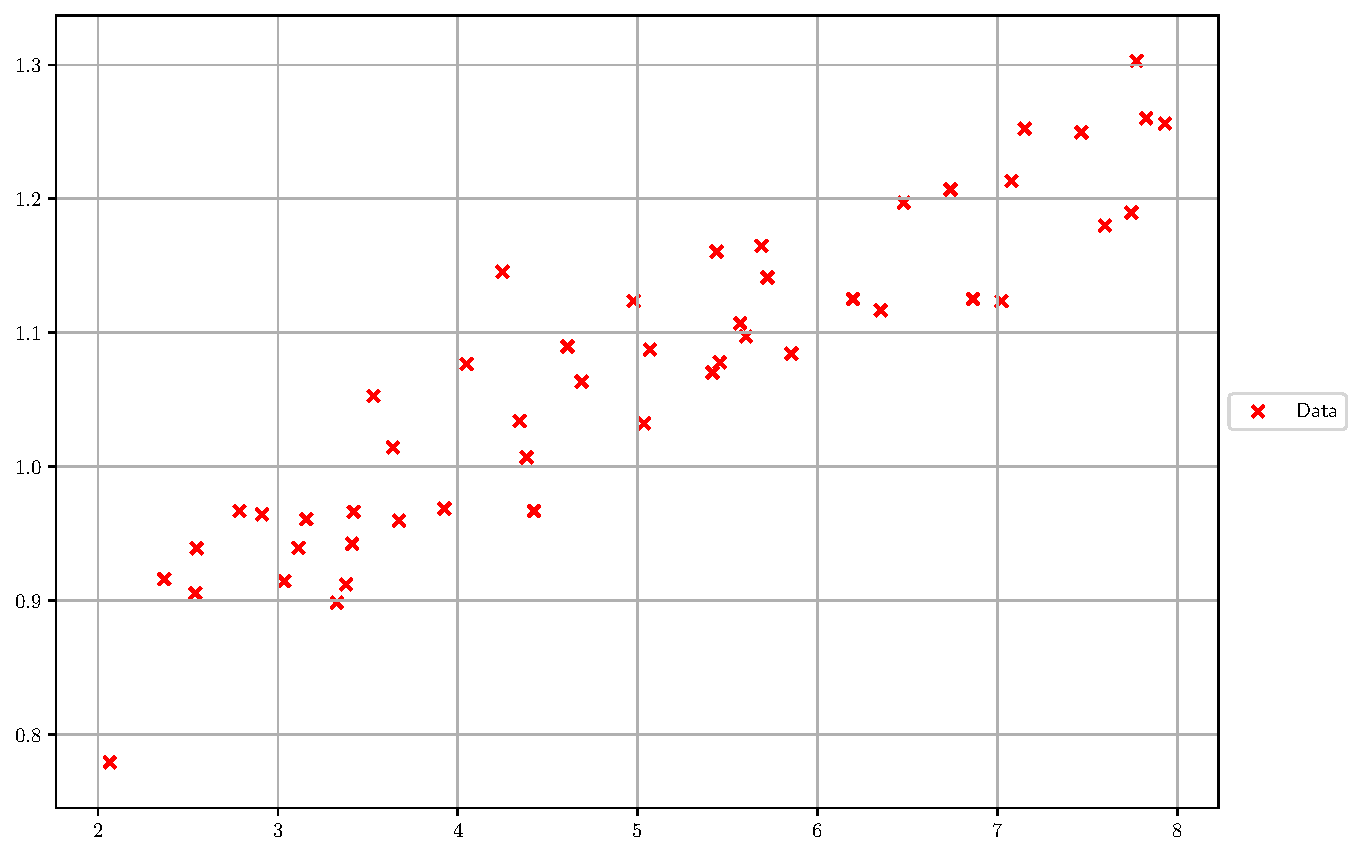
\includegraphics[width=1\textwidth]{../imgs/data.pdf}
    \caption{Dados disponibilizados.}
    \label{fig:data}
\end{figure}
\clearpage

Os valores deste intervalo mencionado acima, foram escolhidos partindo de uma hipótese, 
e a partir desta hipótese, foi possível entender como o \textit{erro} iria se comportar para
aumentar ou diminuir o valor deste $\alpha$. É importante ressaltar, que quanto menor o erro, ou seja,
quanto mais próximo de $0$, melhor será a predição do algoritmo. No melhor caso, onde o erro é $0$, a
predição é perfeita.\\

\textbf{Para todos os testes, os pesos ($\theta$) foram inicializados com $\theta_0, \theta_1$=$(0,0)$ e inicialmente foi-se 
utilizada 100 iterações para observar o comportamento do algoritmo.\\}

Com isso, o primeiro insight obtido após selecionar um valor para o $\alpha$, foi de que era necessário diminuir
ainda mais seu valor, pois o mesmo estava estourando exponecialmente, ou seja, estava se divergindo da solução,
e o que estamos buscando, é um $\alpha$ que se convirja a solução ideal.

\begin{figure}[!h]
    \centering
    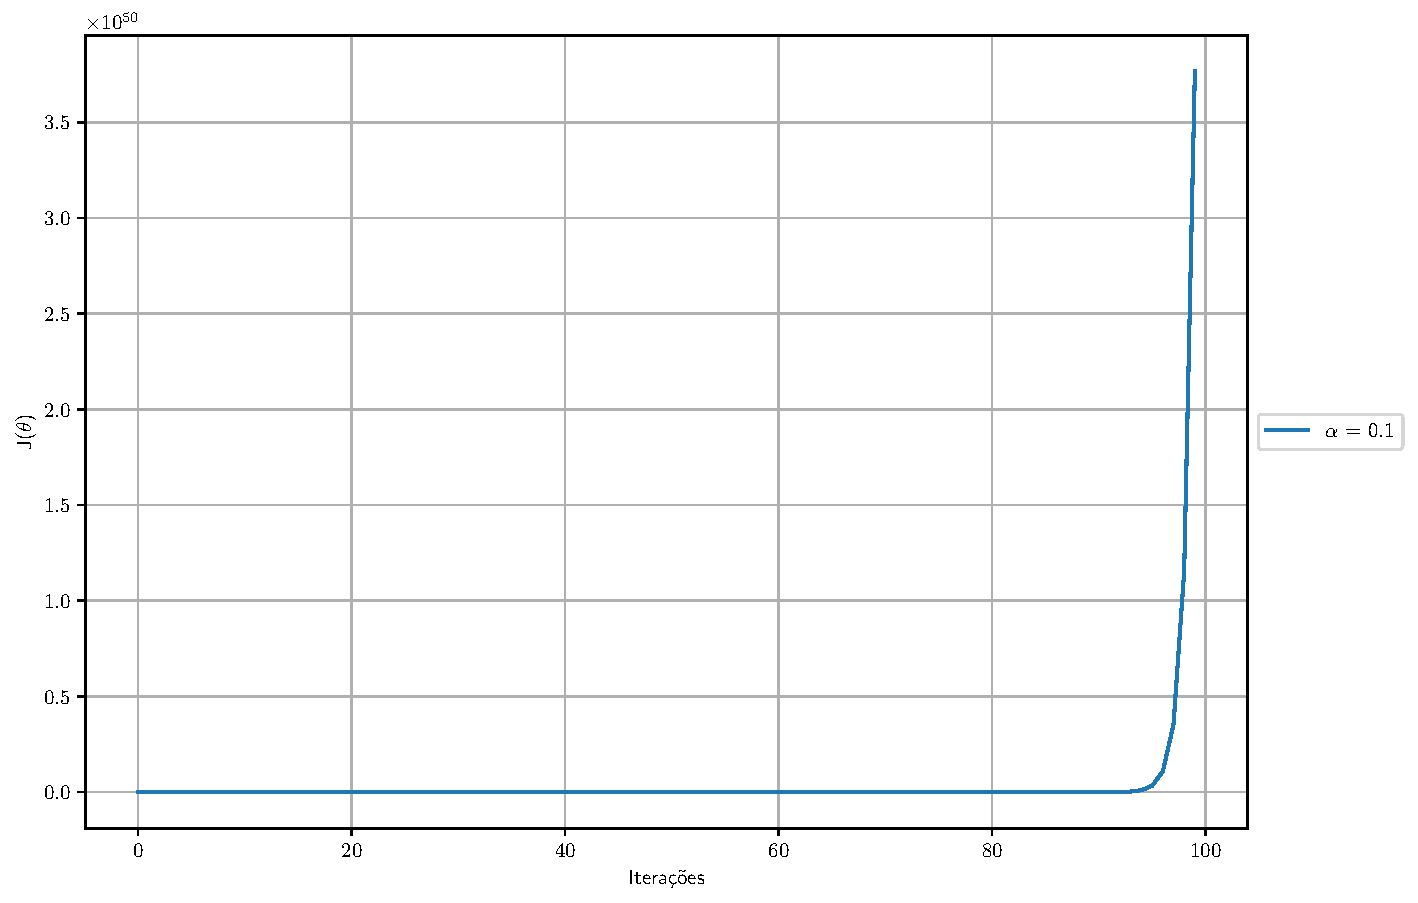
\includegraphics[width=1\textwidth]{../imgs/first_insight.pdf}
    \caption{Primeiro insight obtido a partir de um valor de $\alpha$ inicial.}
    \label{fig:first_insight}
\end{figure}
\clearpage

Com os dados dispostos, se realizarmos a aplicação do algoritmo, utilizando o valor de $\alpha$ acima, que foi de
$0.1$, iremos obter a seguinte predição.
\begin{figure}[!h]
    \centering
    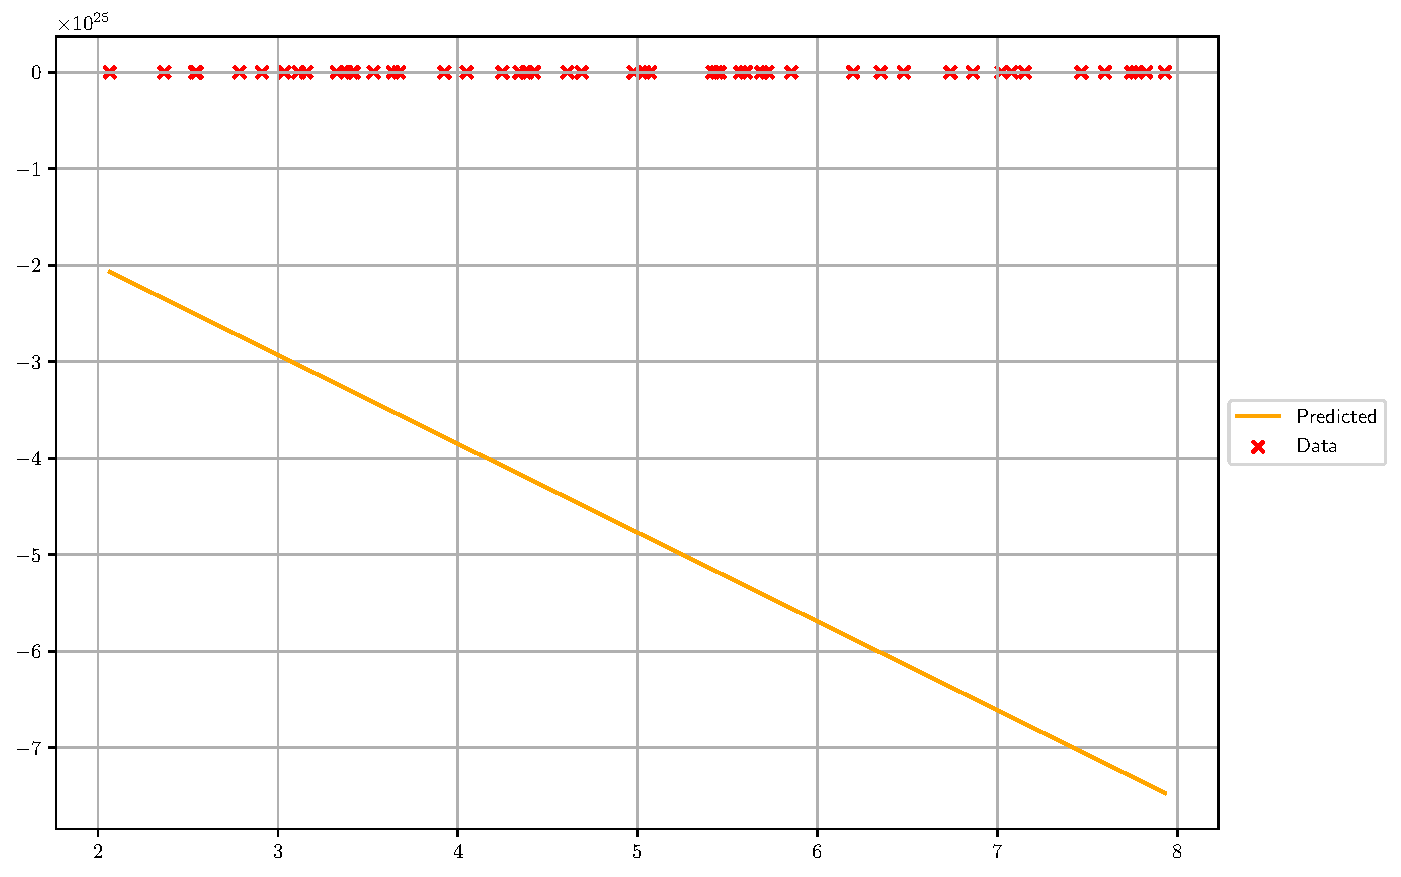
\includegraphics[width=1\textwidth]{../imgs/first_predicted.pdf}
    \caption{Predição com mau treinamento.}
    \label{fig:data}
\end{figure}

Como podemos ver, numa escala logarítmica, a nossa predição está absurdamente longe dos dados que foram
dispostos, aproximadamente $10^{25}$ se comparado no eixo y.
\clearpage

Então, foi realizado alguns testes para tentar selecionar o melhor valor para $\alpha$, logo, é importante
notar que, quanto mais próximo de $0$, melhor será a solução que o algoritmo irá encontrar. 

Neste gráfico, é possivel observar que, para alguns valores de $\alpha$, como o próprio $0.1$, que já foi testado anteriormente, e também,
$0.08$ e $0.09$, convergem da solução e ''estouram'' exponencialmente, portanto esses valores serão descartados para as próximas análises.

É possivel notar também que, para alguns valores temos uma convergência mais rápida, ou seja, essses valores se aproximam mais rápido de $0$; isso significa que, na \textit{Descida de Gradiente}, o algoritmo irá realizar
um salto bem próximo de uma boa solução(valor próximo de $0$), e em contrapartida, alguns valores também convergem, mas de forma mais lenta.

% Este gráfico representa o que conhecemos por \textit{erro}...

\begin{figure}[!h]
    \centering
    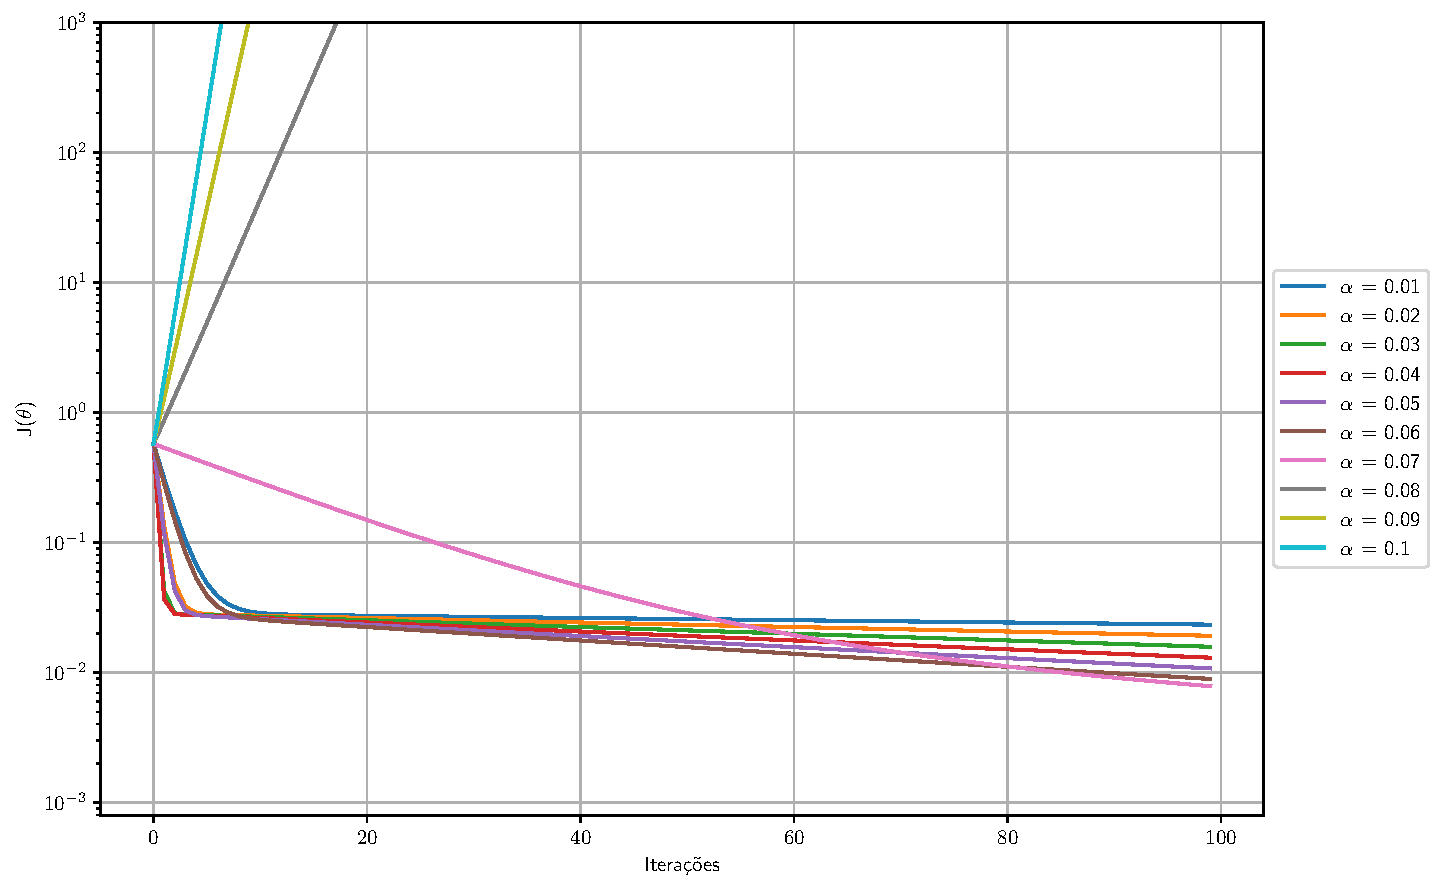
\includegraphics[width=1\textwidth]{../imgs/overflow_insights.pdf}
    \caption{Verificando o erro a partir de diferentes valores de $\alpha$.}
    \label{fig:overflow_insights}
\end{figure}

Logo, a seguinte questão é levantada: ''Para este modelo, o valor de $\alpha$ que converge mais rápido,
será de fato o melhor valor para utilizar no treinamento do algoritmo?''.\\

Para responder essa questão, foi realizado alguns testes para a quantidade atual de iterações e posteriormente será aumentado este
número, para verificar como que o modelo se comporta quando submetido a uma quantidade maior de iterações(treinamento).
\clearpage

No gráfico abaixo, pode-se observar melhor como está atualmente o comportamento do algoritmo para cada
valor de $\alpha$. De primeira impressão, é possivel ver que o valor que mais demora a convergir é $0.07$, porém,
o mesmo é o que está mais próximo do eixo, pode-se afirmar que para 100 iterações, este seria um bom valor,
mas ainda não sabemos se este será de fato o melhor, visto a sua demora a convergir.

Entretanto, não é possivel saber de fato, qual é o valor que converge mais rápido, pois nessa escala, os valores
estão muito próximos um do outro.
\begin{figure}[!h]
    \centering
    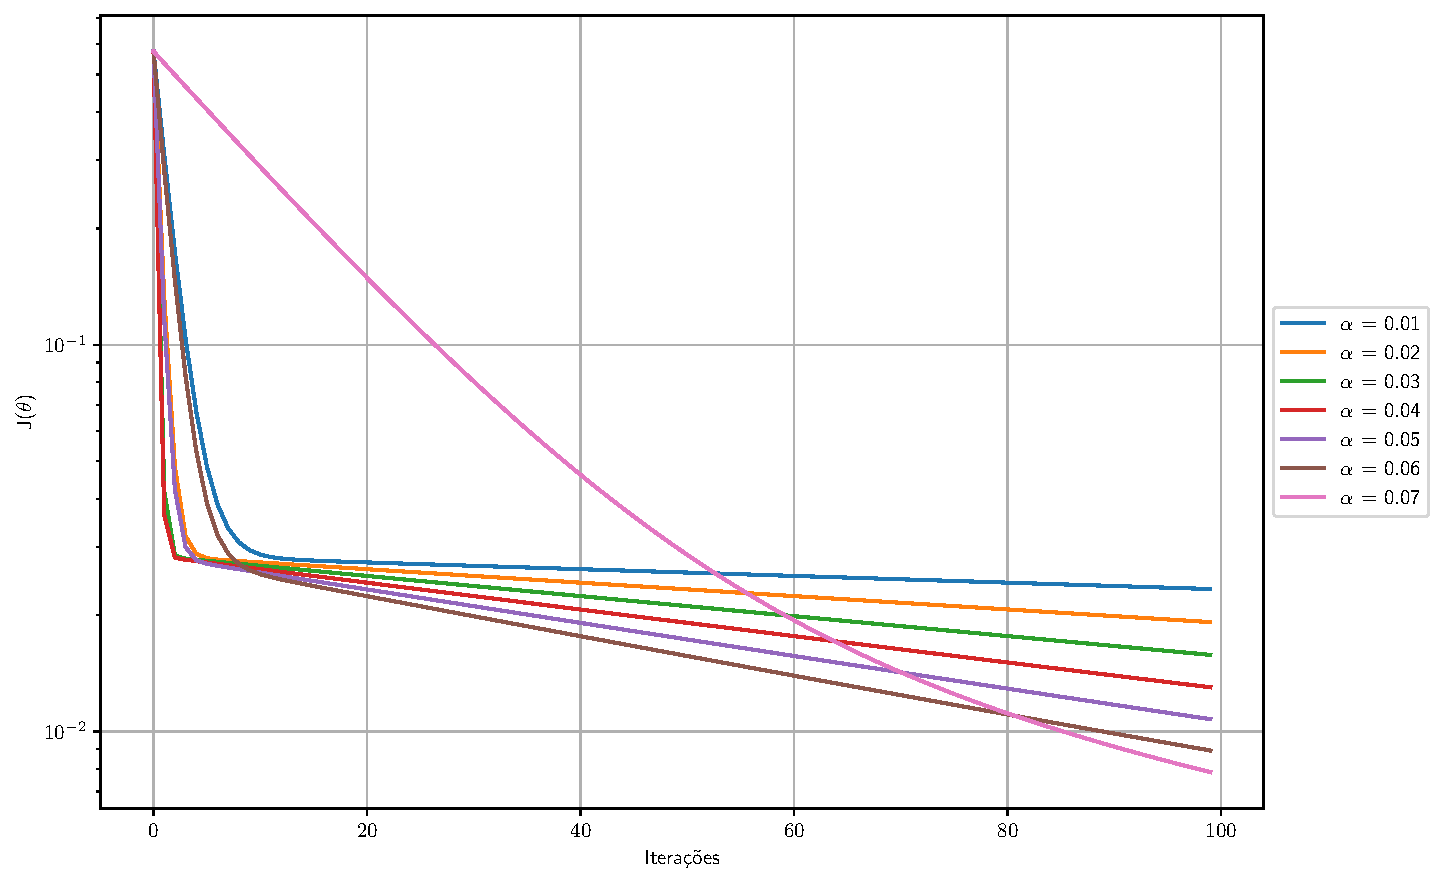
\includegraphics[width=.8\textwidth]{../imgs/lr_100it.pdf}
    \caption{Intervalo de 100 iterações.}
    \label{fig:lr_100it}
\end{figure}

Com isso, o gráfico abaixo foi estreito num intervalo menor, relacionado a figura \ref{fig:lr_100it}. Agora é possível
ver com mais clareza que o valor $0.04$, referente a linha vermelha, é o valor que converge mais rápido. Portanto,
este pode também pode ser considerado um bom valor para realizar o treinamento.
\begin{figure}[!h]
    \centering
    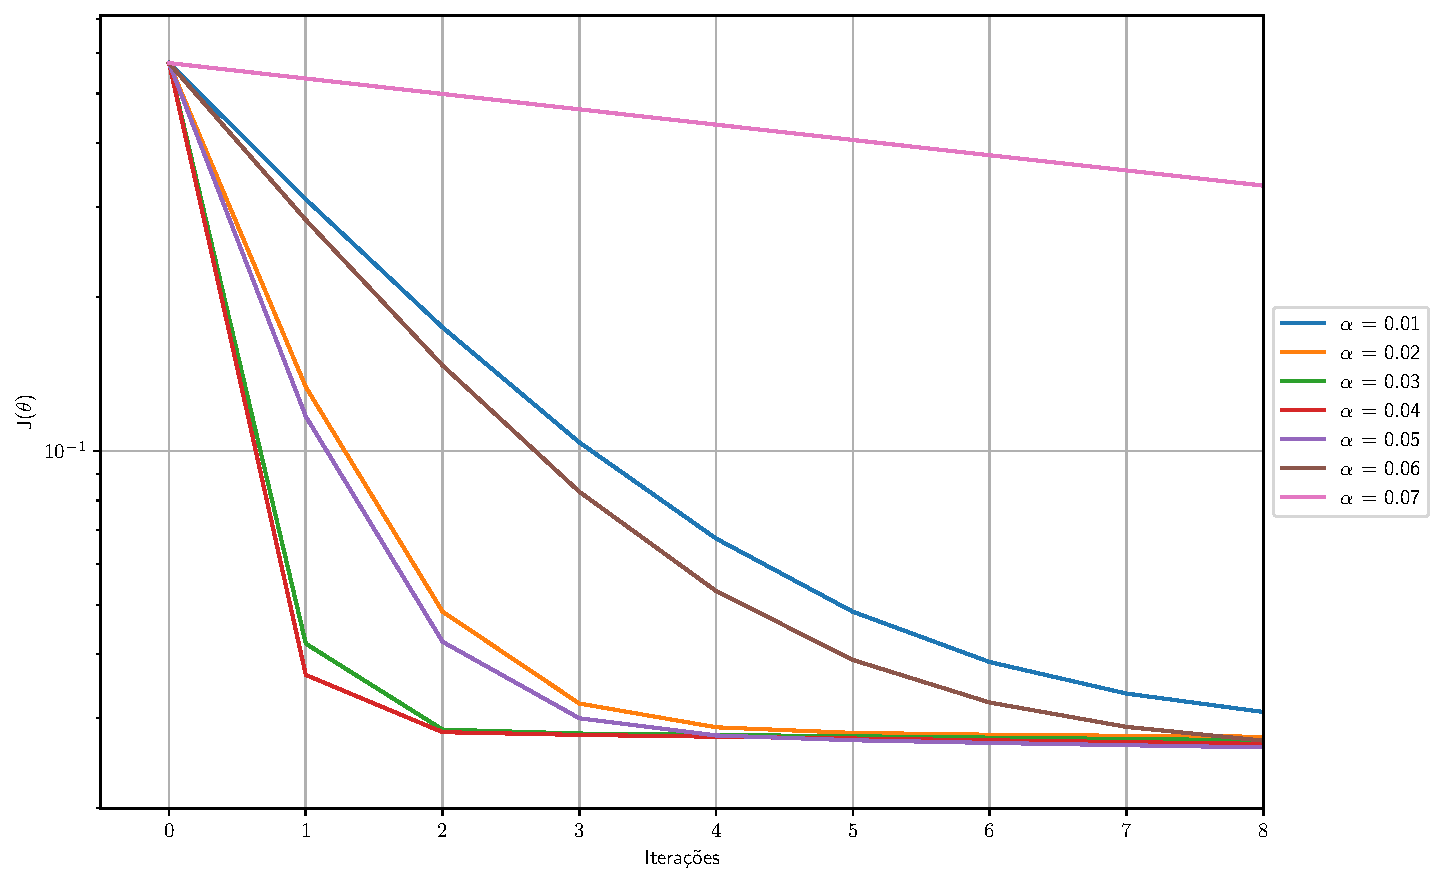
\includegraphics[width=0.8\textwidth]{../imgs/lower_interval.pdf}
    \caption{Intervalo estreito mais a esquerda do eixo.}
    \label{fig:lower_interval}
\end{figure}
\clearpage

Continuando a análise para selecionar o valor de $\alpha$, agora veremos como está se comportando os valores
num intervalo mais restrito ao final do eixo x. Assim como na figura \ref{fig:lr_100it}, como os valores estão
bem diferentes entre si, o comportamento é o mesmo que já foi notado.
\begin{figure}[!h]
    \centering
    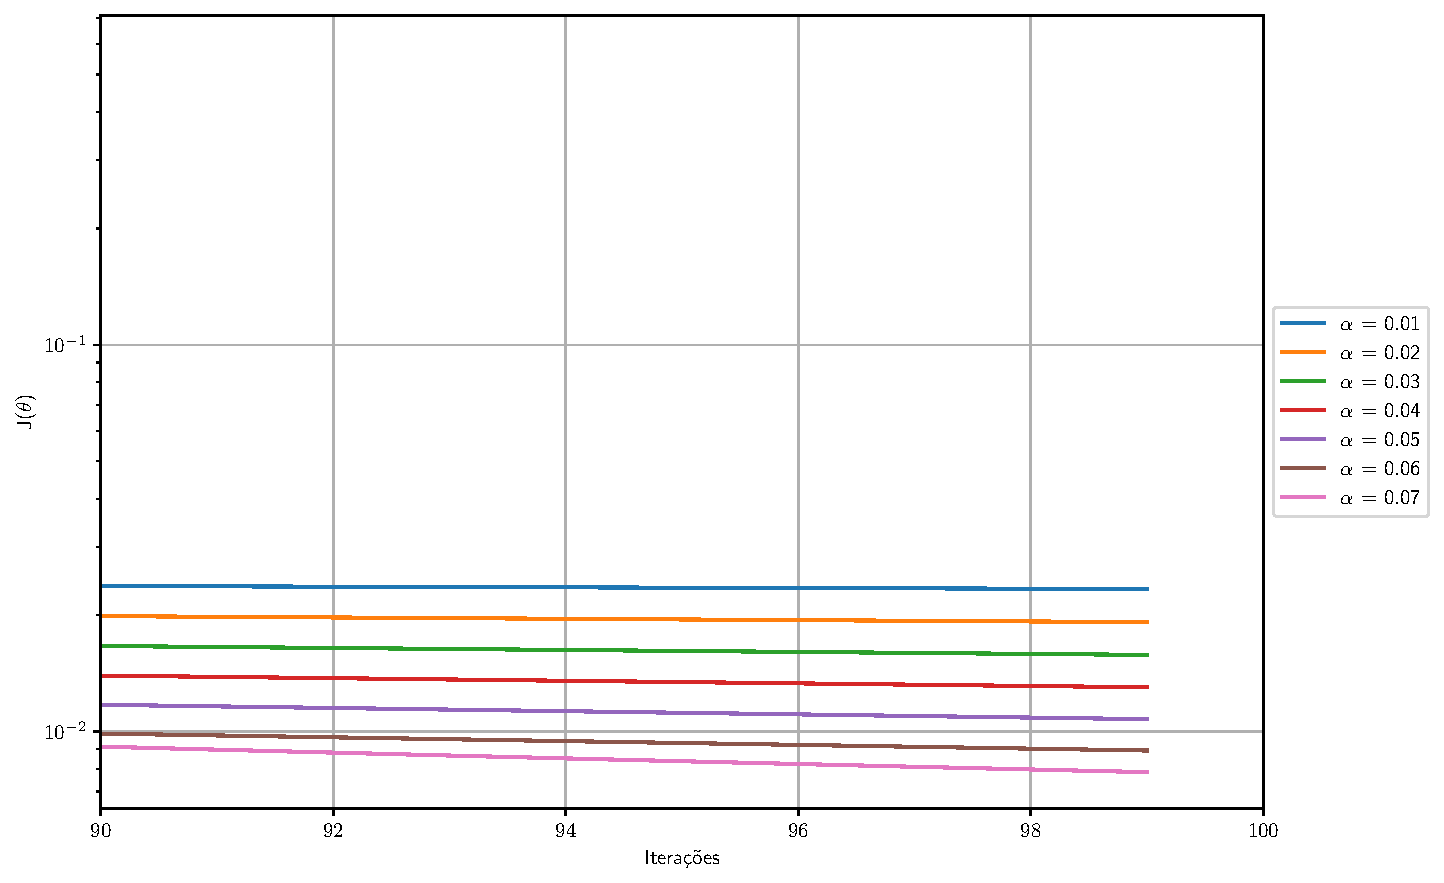
\includegraphics[width=0.8\textwidth]{../imgs/higher_interval_100it.pdf}
    \caption{Intervalo estreito mais a direita do eixo.}
    \label{fig:higher_interval_100it}
\end{figure}

Porém, é importante lembrar que, para este treinamento foi utilizando somente \textbf{100 iterações}, este é um número
pequeno de iterações, mesmo sabendo que os dados dispostos não são tão grandes; porém, para obter uma análise
mais concreta para selecionar um bom $\alpha$ para predizer os valores de y, será realizado outra análise, mas agora
utilizando \textbf{1000 iterações}, e será observado se o comportamento do modelo continua o mesmo, ou se sofre alguma
alteração durante o treinamento.
\clearpage

\subsection{Treinamento utilizando 1000 iterações}

Ao realizar o treinamento utilizando 1000 iterações, pode-se notar que alguns valores de $\alpha$, 
temos alguns valores que convergiram a partir das $500$ iterações e outros não, mesmo que com $100$ iterações,
pareciam ser bons valores, pelo fato de convergir mais rápido que outros valores. 

Logo, podemos afirmar que, não é pelo fato de uma solução convergir mais rápido,
que esta será melhor que as outras, pois ela pode melhorar depois em outro intervalo de iterações.
\begin{figure}[!h]
    \centering
    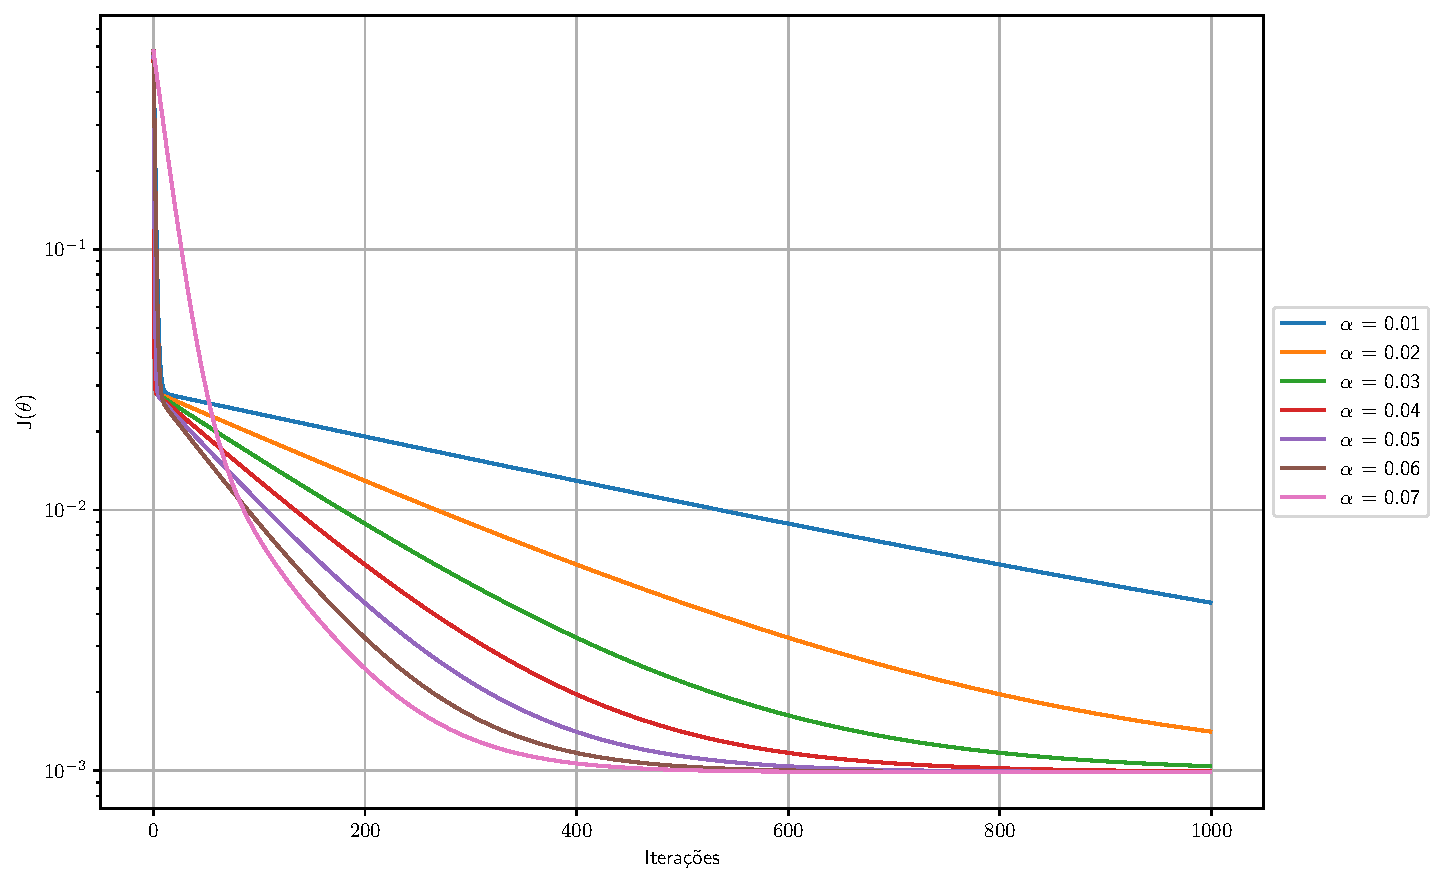
\includegraphics[width=1\textwidth]{../imgs/lr_1000it.pdf}
    \caption{Intervalo de 1000 iterações.}
    \label{fig:lr_100it}
\end{figure}

Porém, novamente, como agora os valores estão muito próximos um do outro, é necessário ampliar o intervalo
ao final do eixo x para saber de fato qual valor está com a menor amplitude em relação ao eixo y. Para isso, foi gerado dois gráficos,
a figura \ref{fig:higher_interval_1000it} e \ref{fig:max_zoom}, as duas figuras estão estreitas no intervalo $[990,1000]$ para $X$, e 
$[10^{-3},10^{-1}]$, $[9.8$ x $10^{-4},1.06$ x $10^{-3}]$, respectivamente.\\

No gráfico da figura \ref{fig:higher_interval_1000it}, é possivel notar a presença de mais de uma linha entre
as cores \textit{verde} e \textit{rosa}, que representam os valores $0.03$ e $0.07$, respectivamente, mas não
dá para distinguir qual valor de fato é este. 

\begin{figure}[!h]
    \centering
    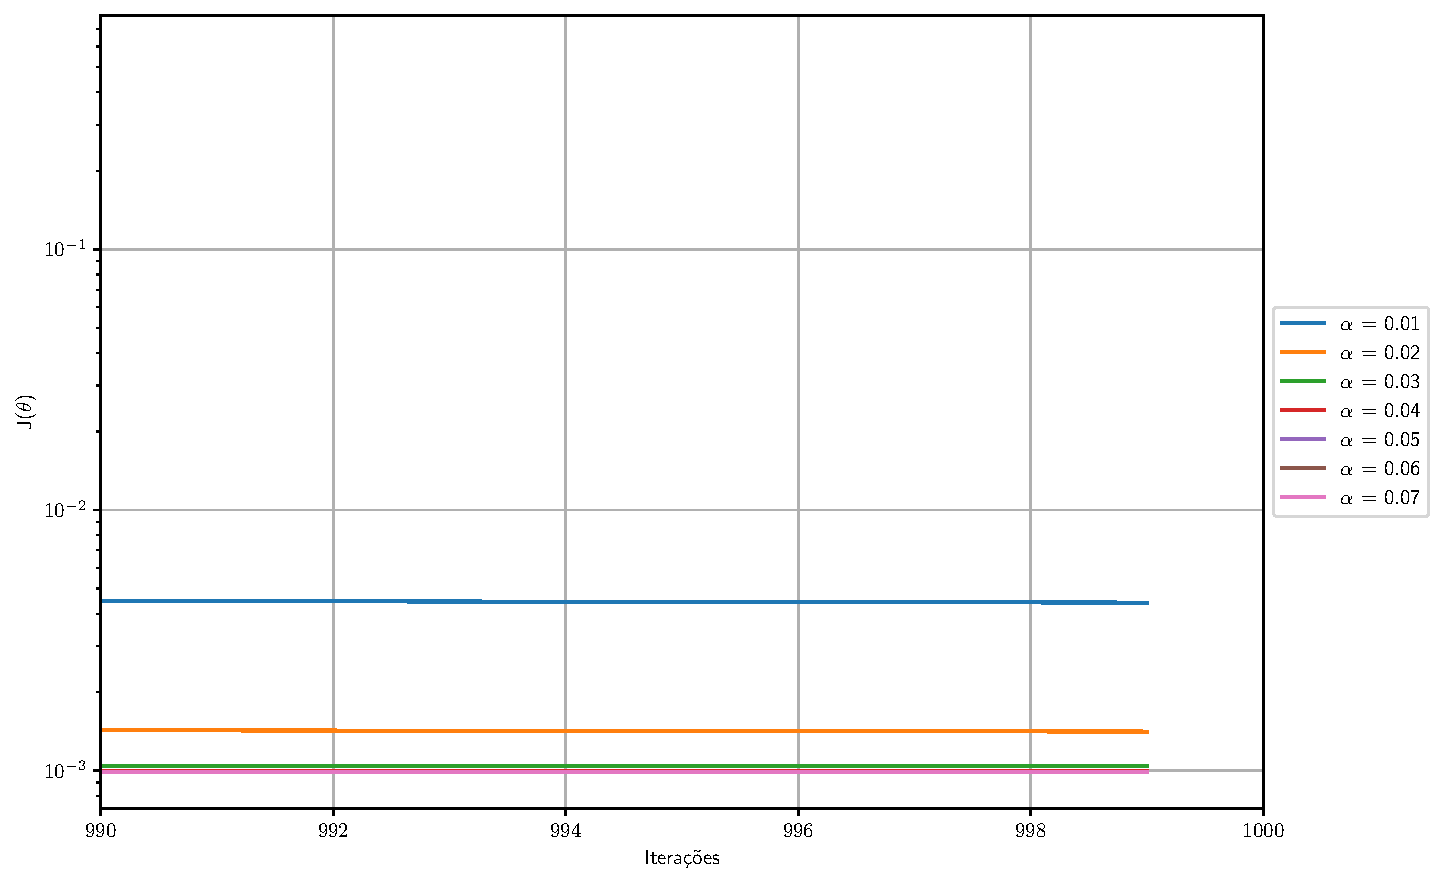
\includegraphics[width=1\textwidth]{../imgs/higher_interval_1000it.pdf}
    \caption{Intervalo estrito mais a direita para 1000 iterações.}
    \label{fig:higher_interval_1000it}
\end{figure}

No gráfico da figura \ref{fig:max_zoom}, é pode-se observar quais são valores presentes neste intervalo, considerando
que este intervalo de y é muito pequeno.

\begin{figure}[!h]
    \centering
    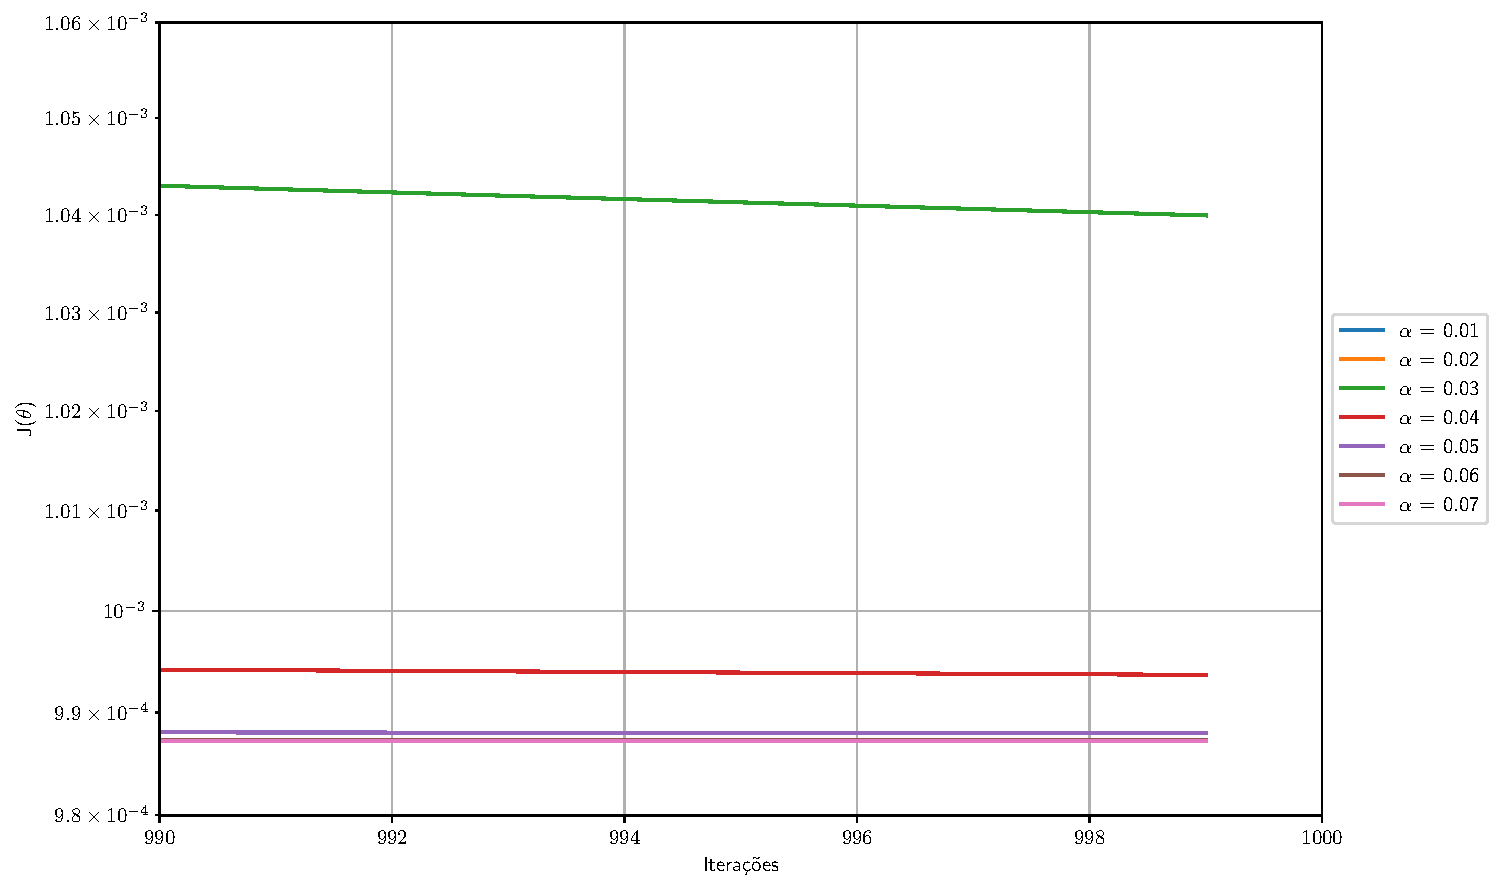
\includegraphics[width=1\textwidth]{../imgs/max_zoom.pdf}
    \caption{Zoom no intervalo.}
    \label{fig:max_zoom}
\end{figure}
\clearpage

\section{Interpretação dos Resultados}
Após estudarmos o comportamento do erro($J(\theta)$) deste modelo para os $\alpha$ selecionados, podemos de fato
selecionar um valor de $\alpha$ global dentre os locais utilizados para estudo. Com o estudo do erro, é 
possivel saber quando teremos um bom e um mau modelo, ou seja, quanto mais divergente do eixo for este erro,
pior será o modelo. 

O gráfico abaixo, mostra as predições para todos os valores de $\alpha$ estudados quando estes convergiam. 

\begin{figure}[!h]
    \centering
    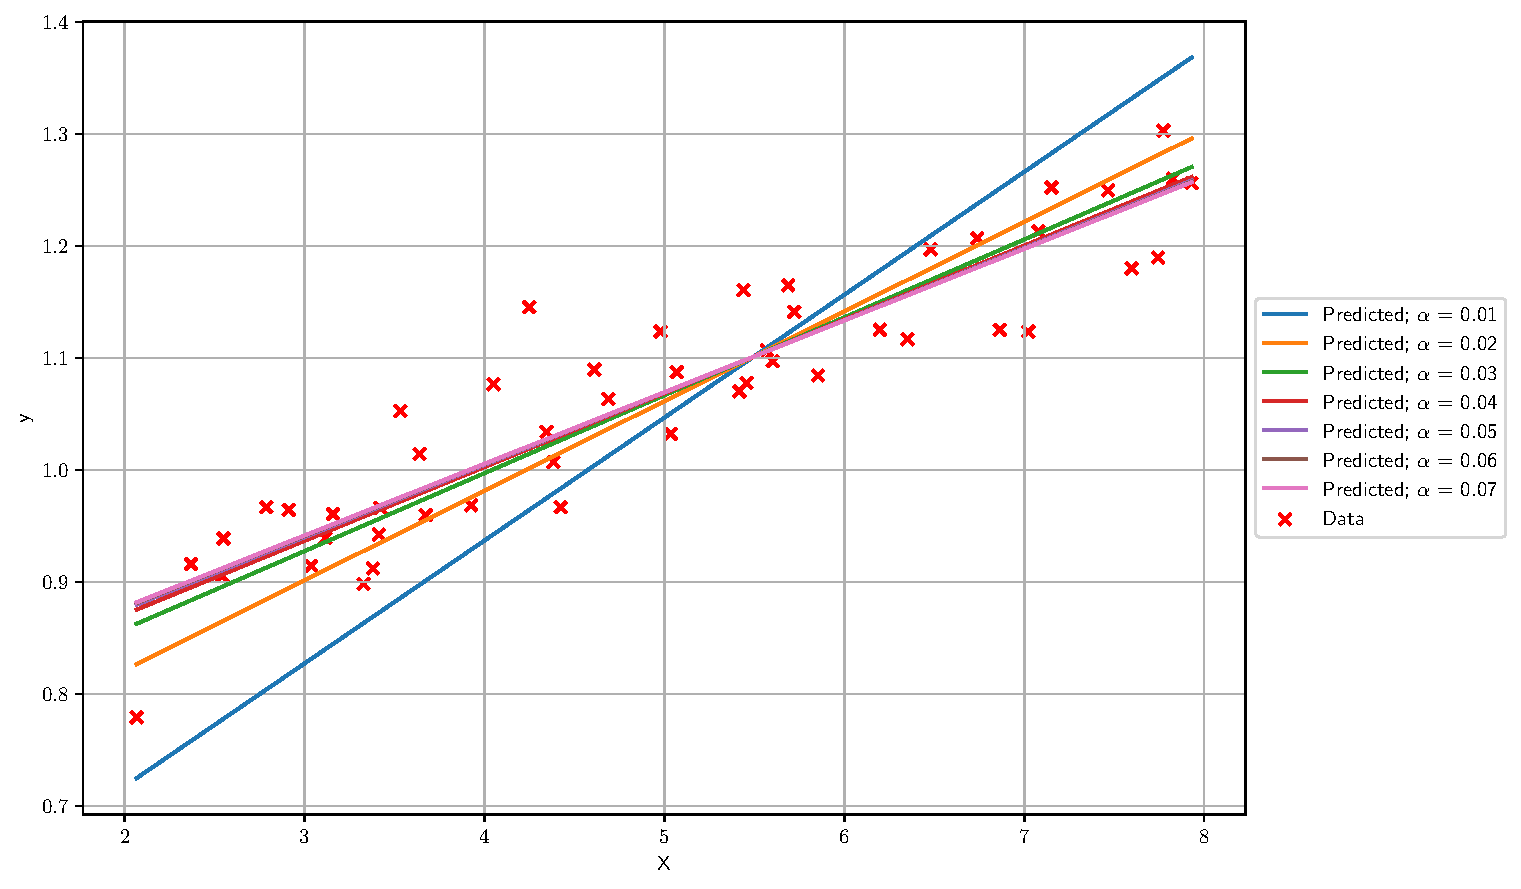
\includegraphics[width=1\textwidth]{../imgs/all_predictions.pdf}
    \caption{Todas as predições para os $\alpha's$ convergentes.}
    \label{fig:all_predictions}
\end{figure}
\clearpage

\section{Conclusão}
Após as análises, podemos ver que o $\alpha$ que mais se mostrou próximo de uma solução exata foi o de valor $0.07$.

Podemos ver que, dispersos no plano temos alguns $outliers$, mas de forma geral, existe uma relação linear entre os dados.
\begin{figure}[!h]
    \centering
    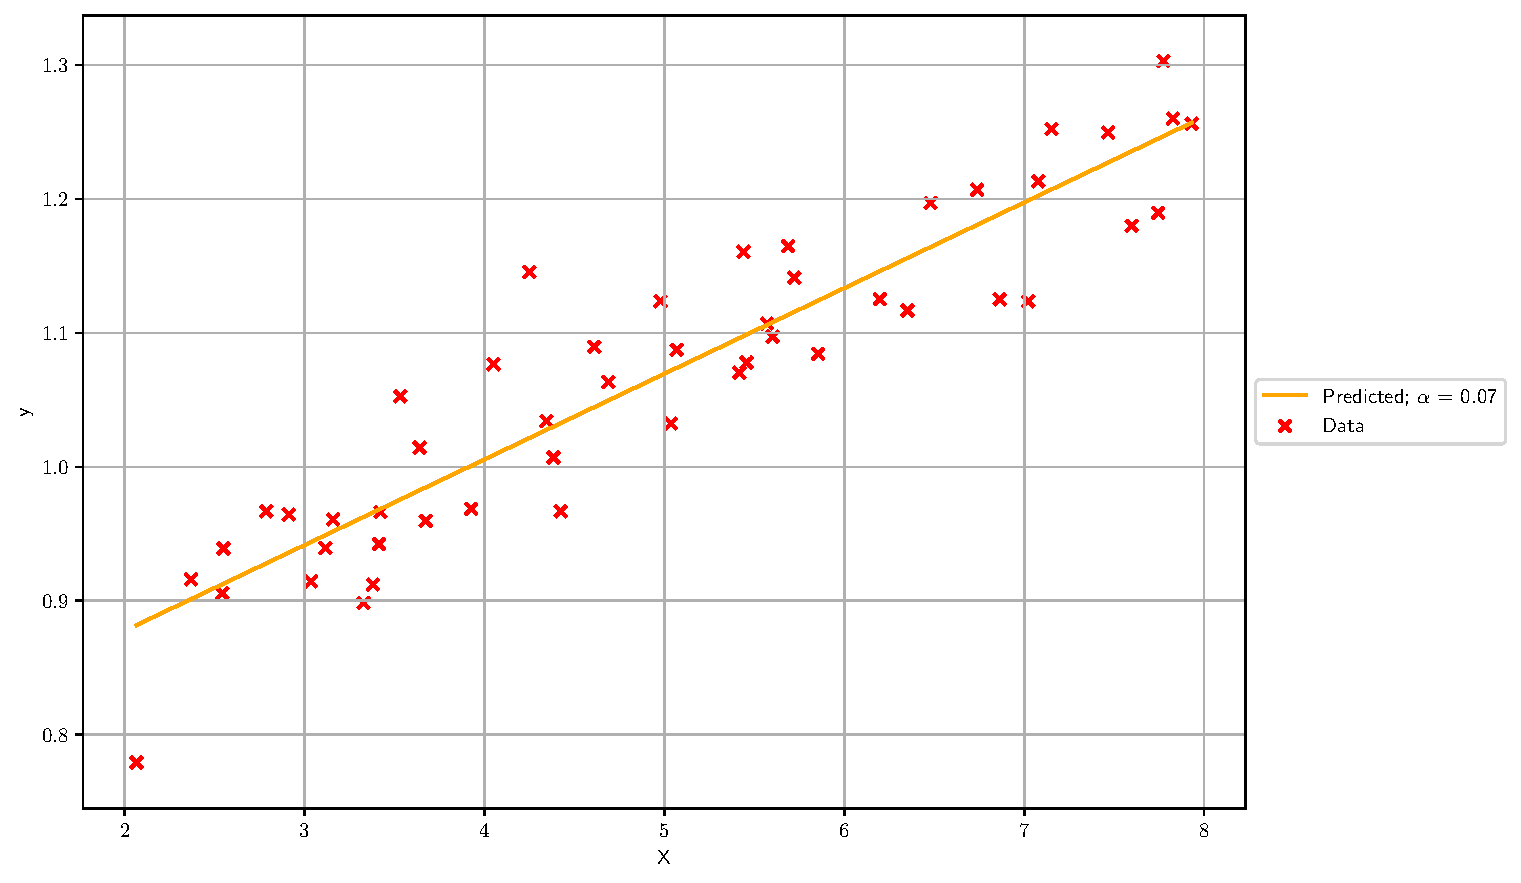
\includegraphics[width=1\textwidth]{../imgs/FINAL_predicted.pdf}
    \caption{Modelo final.}
    \label{fig:FINAL_predicted}
\end{figure}

\end{document}